\begin{frame}
    \frametitle{Documental}

    Las bases de datos documentales almacenan datos en documentos individuales, que pueden ser estructurados o semi-estructurados como archivos JSON o XML.
    
    \begin{center}
    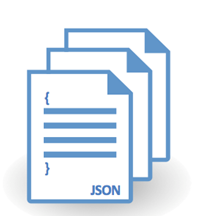
\includegraphics[width=0.2\textwidth]{diagramas/Documental.png}
    \end{center}
\end{frame}

\begin{frame}
    \frametitle{Documental - Ventajas}

    \begin{itemize}
        \item Las bases de datos son flexibles.  
        \item Los sistemas pueden crear índices sobre algunos elementos de datos para mejorar el rendimiento de las consultas.
    \end{itemize}
\end{frame}

\begin{frame}
    \frametitle{Documental - Casos de uso}
    Las bases de datos documentales son especialmente adecuadas para aplicaciones donde los datos tienen una estructura flexible y variable como por ejemplo:
    
     
    
    \begin{itemize}
        \item Contenido web  
        \item Análisis de registros  
        \item Gestión de datos de productos
    \end{itemize}
\end{frame}

\begin{frame}
    \frametitle{Documental - Ejemplos}
    \begin{itemize}
        \item \textbf{MongoDB}\\
        Es una base de datos documental líder que utiliza un modelo de datos basado en documentos JSON. Ofrece capacidad de escalabilidad horizontal y opciones avanzadas de replicación, lo que permite gestionar grandes cantidades de datos y cargas de trabajo exigentes.

         

        \item \textbf{CouchDB}\\
        Se destaca por su simplicidad en la replicación y consulta. Utiliza un modelo de datos basado en documentos JSON y es especialmente adecuado para cargas de trabajo menos intensivas y entornos donde la replicación descentralizada es una necesidad.
    \end{itemize}
\end{frame}